% Sección 8.5: Ejercicios

\subsection*{SECCIÓN 8.5 \quad Ejercicios}

\begin{enumerate}
    \subimport{ejercicio_01/}{ejercicio.tex}
\subimport{ejercicio_02/}{ejercicio.tex}
\end{enumerate}

\vspace{0.3cm}
\noindent\textit{En los ejercicios 3-12 se tiene un tanque que contiene agua. El extremo del tanque es vertical y tiene la forma indicada. Encuentre la fuerza hidrostática que actúa en contra del extremo del tanque.}

\begin{enumerate}
    \setcounter{enumi}{2}
    \subimport{ejercicio_03/}{ejercicio.tex}
\vspace{0.2cm}
    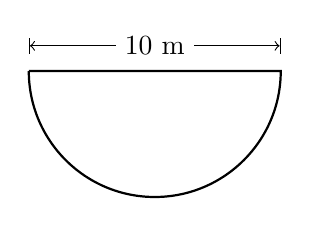
\begin{tikzpicture}[scale=0.8]
        \draw[thick] (-2,0) -- (2,0) arc (0:-180:2);
        \draw[|<->|] (-2,0.4) -- (2,0.4) node[midway, fill=white] {10 m};
    \end{tikzpicture}
    
    \subimport{ejercicio_04/}{ejercicio.tex}
\vspace{0.2cm}
    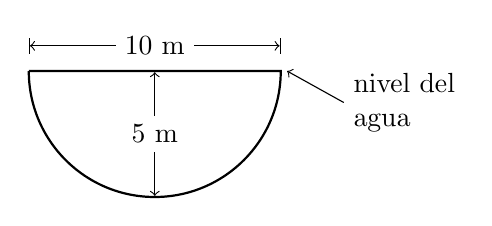
\begin{tikzpicture}[scale=0.8]
        \draw[thick] (-2,0) -- (2,0) arc (0:-180:2);
        \draw[|<->|] (-2,0.4) -- (2,0.4) node[midway, fill=white] {10 m};
        \draw[|<->|] (0,0) -- (0,-2) node[midway, fill=white] {5 m};
        \draw[<-] (2.1,0) -- (3, -0.5) node[right, align=left] {nivel del\\agua};
    \end{tikzpicture}

    \subimport{ejercicio_05/}{ejercicio.tex}
\vspace{0.2cm}
    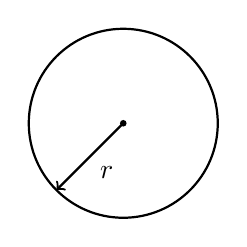
\begin{tikzpicture}[scale=0.8]
        \draw[thick] (0,0) circle (1.5);
        \fill (0,0) circle (1.5pt);
        \draw[->, thick] (0,0) -- (-1.06, -1.06) node[midway, below right] {$r$};
    \end{tikzpicture}

    \subimport{ejercicio_06/}{ejercicio.tex}
\vspace{0.2cm}
    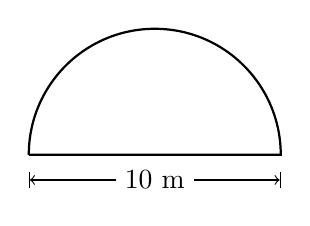
\begin{tikzpicture}[scale=0.8]
        \draw[thick] (-2,0) -- (2,0) arc (0:180:2);
        \draw[|<->|] (-2,-0.4) -- (2,-0.4) node[midway, fill=white] {10 m};
    \end{tikzpicture}

    \subimport{ejercicio_07/}{ejercicio.tex}
\vspace{0.2cm}
    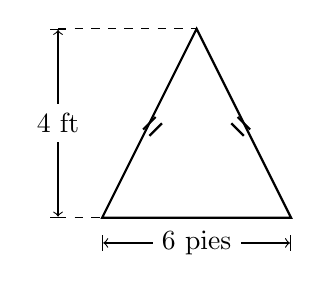
\begin{tikzpicture}[scale=0.8]
        \draw[thick] (-1.5,0) -- (1.5,0) -- (0,3) -- cycle;
        % Marcas de isósceles
        \draw[thick] (-0.85, 1.4) -- (-0.65, 1.6);
        \draw[thick] (-0.75, 1.3) -- (-0.55, 1.5);
        \draw[thick] (0.85, 1.4) -- (0.65, 1.6);
        \draw[thick] (0.75, 1.3) -- (0.55, 1.5);
        % Cotas
        \draw[|<->|] (-1.5,-0.4) -- (1.5,-0.4) node[midway, fill=white] {6 pies};
        \draw[|<->|] (-2.2,0) -- (-2.2,3) node[midway, fill=white] {4 ft};
        \draw[dashed] (-2.2,0) -- (-1.5,0);
        \draw[dashed] (-2.2,3) -- (0,3);
    \end{tikzpicture}

    \subimport{ejercicio_08/}{ejercicio.tex}
\vspace{0.2cm}
    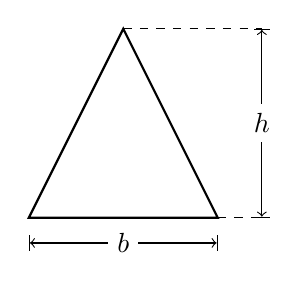
\begin{tikzpicture}[scale=0.8]
        \draw[thick] (-1.5,0) -- (1.5,0) -- (0,3) -- cycle;
        \draw[|<->|] (-1.5,-0.4) -- (1.5,-0.4) node[midway, fill=white] {$b$};
        \draw[|<->|] (2.2,0) -- (2.2,3) node[midway, fill=white] {$h$};
        \draw[dashed] (1.5,0) -- (2.2,0);
        \draw[dashed] (0,3) -- (2.2,3);
    \end{tikzpicture}

    \subimport{ejercicio_09/}{ejercicio.tex}
\vspace{0.2cm}
    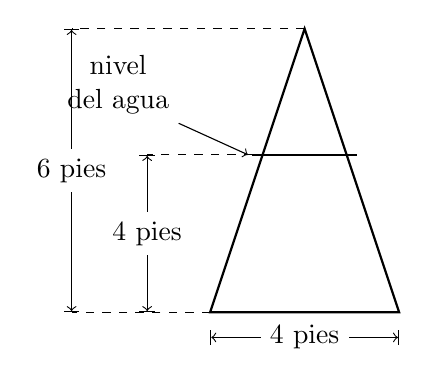
\begin{tikzpicture}[scale=0.8]
        \draw[thick] (-1.5, 0) -- (1.5, 0) -- (0, 4.5) -- cycle;
        \draw[thick] (-0.83, 2.5) -- (0.83, 2.5); % Nivel del agua
        \draw[<-] (-0.9, 2.5) -- (-2, 3) node[above left, align=center] {nivel\\del agua};
        \draw[|<->|] (-1.5, -0.4) -- (1.5, -0.4) node[midway, fill=white] {4 pies};
        \draw[|<->|] (-2.5, 0) -- (-2.5, 2.5) node[midway, fill=white] {4 pies};
        \draw[|<->|] (-3.7, 0) -- (-3.7, 4.5) node[midway, fill=white] {6 pies};
        \draw[dashed] (-1.5, 0) -- (-3.7, 0);
        \draw[dashed] (-0.83, 2.5) -- (-2.5, 2.5);
        \draw[dashed] (0, 4.5) -- (-3.7, 4.5);
    \end{tikzpicture}

    \subimport{ejercicio_10/}{ejercicio.tex}
\vspace{0.2cm}
    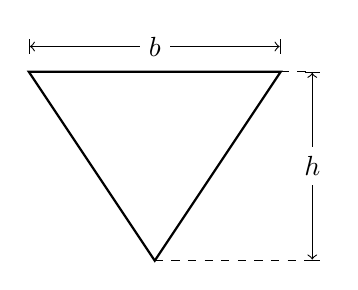
\begin{tikzpicture}[scale=0.8]
        \draw[thick] (-2,3) -- (2,3) -- (0,0) -- cycle;
        \draw[|<->|] (-2,3.4) -- (2,3.4) node[midway, fill=white] {$b$};
        \draw[|<->|] (2.5,0) -- (2.5,3) node[midway, fill=white] {$h$};
        \draw[dashed] (0,0) -- (2.5,0);
        \draw[dashed] (2,3) -- (2.5,3);
    \end{tikzpicture}

    \subimport{ejercicio_11/}{ejercicio.tex}
\vspace{0.2cm}
    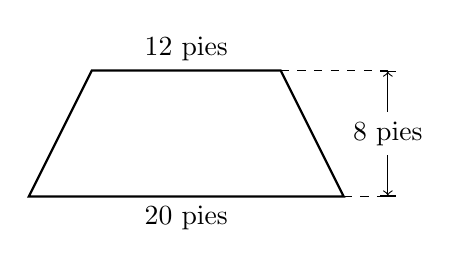
\begin{tikzpicture}[scale=0.8]
        \draw[thick] (-1.5, 2) -- (1.5, 2) -- (2.5, 0) -- (-2.5, 0) -- cycle;
        \node[above] at (0, 2) {12 pies};
        \node[below] at (0, 0) {20 pies};
        \draw[dashed] (1.5, 2) -- (3.2, 2);
        \draw[dashed] (2.5, 0) -- (3.2, 0);
        \draw[|<->|] (3.2, 0) -- (3.2, 2) node[midway, fill=white] {8 pies};
    \end{tikzpicture}

    \subimport{ejercicio_12/}{ejercicio.tex}
\vspace{0.2cm}
    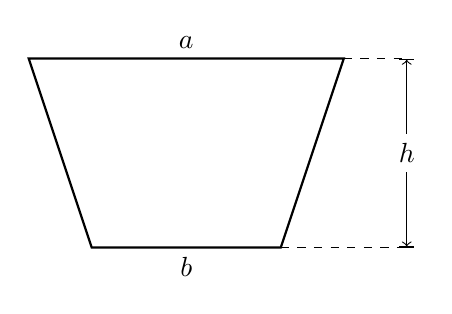
\begin{tikzpicture}[scale=0.8]
        \draw[thick] (-2.5, 3) -- (2.5, 3) -- (1.5, 0) -- (-1.5, 0) -- cycle;
        \node[above] at (0, 3) {$a$};
        \node[below] at (0, 0) {$b$};
        \draw[dashed] (2.5, 3) -- (3.5, 3);
        \draw[dashed] (1.5, 0) -- (3.5, 0);
        \draw[|<->|] (3.5, 0) -- (3.5, 3) node[midway, fill=white] {$h$};
    \end{tikzpicture}
\end{enumerate}

\vspace{0.5cm}
\begin{enumerate}
    \setcounter{enumi}{12}
    \subimport{ejercicio_13/}{ejercicio.tex}
\subimport{ejercicio_14/}{ejercicio.tex}
\subimport{ejercicio_15/}{ejercicio.tex}
\subimport{ejercicio_16/}{ejercicio.tex}
\subimport{ejercicio_17/}{ejercicio.tex}
\subimport{ejercicio_18/}{ejercicio.tex}
\subimport{ejercicio_19/}{ejercicio.tex}
\subimport{ejercicio_20/}{ejercicio.tex}
\subimport{ejercicio_21/}{ejercicio.tex}
\subimport{ejercicio_22/}{ejercicio.tex}
\end{enumerate}
